\documentclass{exam}
\usepackage[body={20cm, 25cm}]{geometry}
\usepackage[spanish]{babel}
\usepackage[utf8]{inputenc}					% include acents
%\usepackage[ansinew,latin1]{inputenc}
\usepackage[OT1]{fontenc}
\usepackage{amsmath,amssymb}
\usepackage{graphicx} % Para insertar y manejar imagenes
%\usepackage{subfig}
\usepackage{float}
\usepackage{caption}
\usepackage{subcaption}
\usepackage{enumerate}
\usepackage{enumitem} % Para usar [resume] en la enumeracion
\usepackage{cleveref}
\decimalpoint
%\usepackage{wrapfig}
%

%%% COMIENZO DE DOCUMENTO %%%
\begin{document}
\pagestyle{empty}
%%% Encabezado


\begin{center}
	{\huge Mecánica de medios continuos avanzada - Trabajo final }\\
	
	{\Large Empujes sobre una presa de concreto}
\end{center}

En la \cref{presa} se muestra una presa triangular sometida a los empujes de un fluido. El ángulo interno es $\phi = \pi/4$.

\begin{figure}[H]
	\centering
	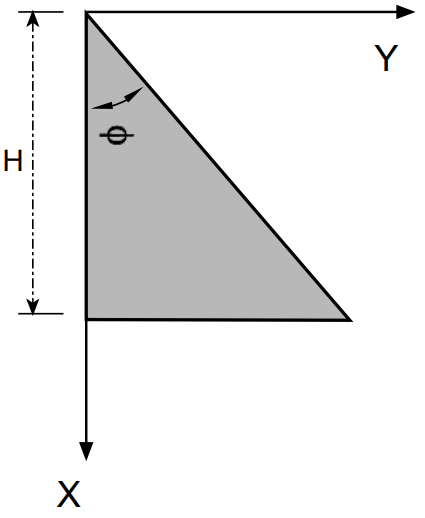
\includegraphics[height=5.5cm]{images/presa.PNG}
	\caption{Presa triangular sometida a los empujes de un fluido}
	\label{presa}
\end{figure}

Dicha presa se ve sometida al siguiente estado de esfuerzos en dos dimensiones:

\begin{eqnarray*}
\sigma_{xx} = \gamma x - 2 \gamma y \\
\sigma_{yy} = - \gamma x \\
\tau_{xy} = - \gamma y
\end{eqnarray*}

donde $\gamma$ representa el peso específico del fluido contenido por la presa. \\

Con esa información, se debe realizar lo siguiente:

\begin{enumerate}
	\item Graficar los esfuerzos sobre la presa. Los tres esfuerzos se visualizan de manera independiente. Ayuda: las gráficas finales debe parecerse a las presentadas en la figura 4.12 de las notas de clase.
	
	\item Calcular los esfuerzos máximos (compresión, tracción y cortante) y su ubicación en la presa.
	
	\item Graficar los esfuerzos máximos (compresión, tracción y cortante) en toda la presa. Se hace un procedimiento análogo al del numeral 1, pero esta vez se usan los esfuerzos principales ($\sigma_1, \sigma_2, \tau_{max}$) como campos para graficar. Para tal fin, los parámetros del círculo de Mohr, centro y radio, se calculan en función de las coordenadas.
	
	\item Suponga que la presa se va a fabricar de concreto y se necesita identificar las zonas de la presa donde hay compresión y donde hay tracción. Grafique dichas zonas de manera diferenciada.
	
	\item Analice la solución de esta presa y \textbf{argumente} si es posible cambiar las zonas de compresión y tracción identificadas previamente, mediante la variación de sus parámetros (altura $H$ y pero específico del fuido $\gamma$).
	
\end{enumerate} 

\vspace{0.5cm}
\textbf{Notas:}
\begin{itemize}
	\item El documento entregado debe ser autocontenido, es decir, que se lea y tenga sentido por sí solo sin referenciar otros documentos.
	\item El trabajo se tiene que entregar el viernes 29 de marzo a las 2:00pm o antes.
	\item Una inadecuada presentación del trabajo causa una penalización del 30\% en la nota obtenida.
	\item Cada numeral tiene un valor del 20\% sobre la nota final.
	\item Se debe realizar en grupos de 3 personas.
	\item El trabajo tiene una fuerte componente de programación, por lo que se recomienda que haya al menos un integrante del grupo que esté familiarizado con temas de programación y visualización.
	\item Se sugiere \textit{Python} para resolver el trabajo, pero se admiten gráficas generadas en cualquier lenguaje o programa.
	\item En las gráficas de las notas de clase se usan contornos. Se puede usar cualquier otra manera de graficar, siempre y cuando se entiendan los resultados.
\end{itemize}

\end{document}